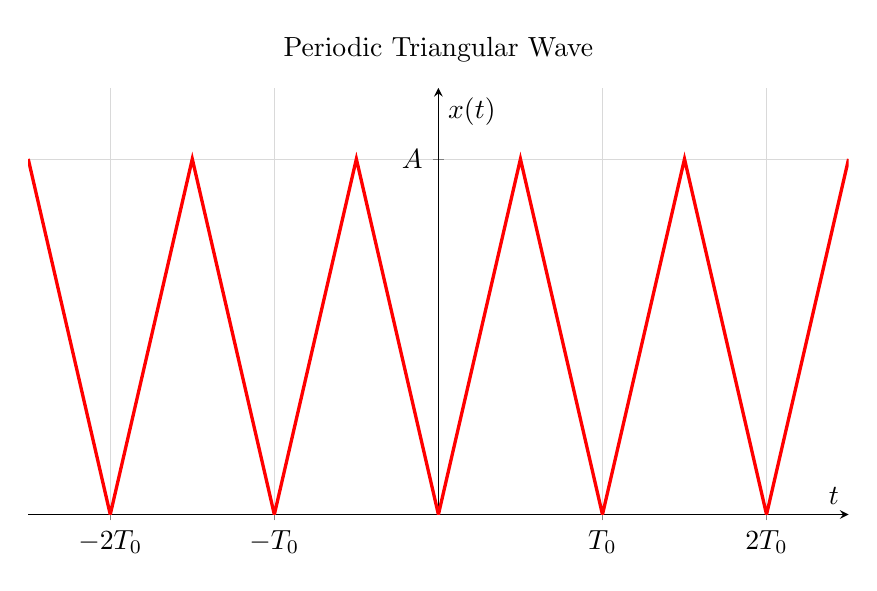
\begin{tikzpicture}
	\begin{axis}[
		width=12cm,
		height=7cm,
		axis lines=middle,
		xlabel={$t$},
		ylabel={$x(t)$},
		title={Periodic Triangular Wave},
		xmin=-5, xmax=5,
		ymin=0, ymax=1.2,
		xtick={-4, -2, 2, 4},
		xticklabels={$-2T_0$, $-T_0$, $T_0$, $2T_0$},
		ytick={1},
		yticklabels={$A$},
		grid=major,
		grid style={line width=.1pt, draw=gray!30},
		]
		
		% Plot the triangular wave
		\draw[red, very thick]
		(axis cs:-5,1) -- (axis cs:-4,0) -- (axis cs:-3,1) -- (axis cs:-2,0)
		-- (axis cs:-1,1) -- (axis cs:0,0) -- (axis cs:1,1) -- (axis cs:2,0)
		-- (axis cs:3,1) -- (axis cs:4,0) -- (axis cs:5,1);
		
		% Add a single, clear period label
		\draw[<->, thick] (axis cs:0, -0.15) -- (axis cs:2, -0.15) node[midway, below=2pt] {Period $T_0$};
		
	\end{axis}
\end{tikzpicture}